\section{The Fast Fourier Transform}

We begin this review by looking at the waveform shown in Figure \ref{fig:FFT Sample Waveform}.
When we take the Fast Fourier Transform (FFT) of this signal, we get an output that is complex and exactly the same length.
Since the FFT algorithm doesn't know what our sampling frequency is, we must create our own frequency array. We do so by creating a linear array of numbers between zero and one that is equal in length to the length of the original waveform (which is equal in length to the FFT output).
We then multiply this array by the sampling frequency so that our results range between zero and out sampling frequency.
This calculation is shown in Equation \ref{eq:Create Frequency Array For FFT}.

\begin{equation} \label{eq:Create Frequency Array For FFT}
    f = \text{fs * linspace(0,1,length(waveform))}
\end{equation}

where

\begin{itemize}
    \item fs = sampling frequency
    \item linspace = a common command in many programming languages, used to create a linear array between two numbers
    \item waveform = the original waveform
\end{itemize}

\begin{figure}[H]
    \centering
    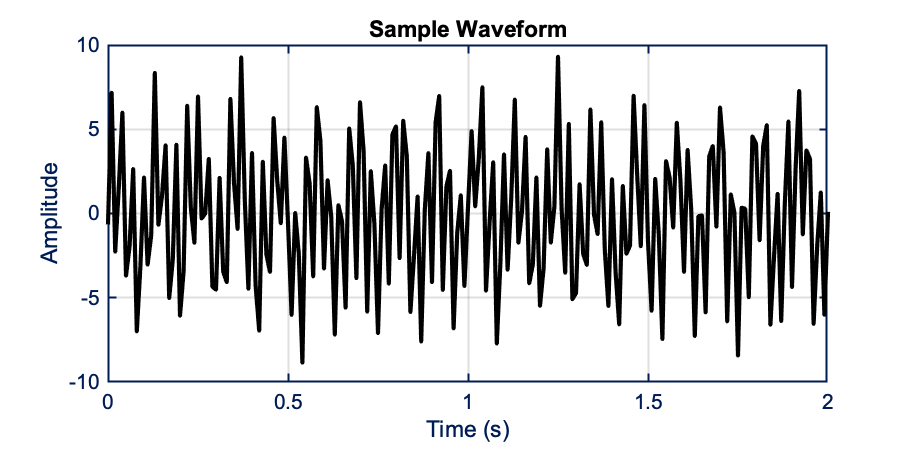
\includegraphics[width = 6 in]{Chapters/Signal Processing/Figures/Sample Waveform.png}
    \caption{A sample waveform for use in the FFT review. I have placed tones at 9 and 33 Hz with amplitudes of 3.0 and 5.0 respectively, along with gaussian-distributed random noise. The sampling frequency is 100 Hz.}
    \label{fig:FFT Sample Waveform}
\end{figure}

Once this frequency array is created, we can start looking at the output.
For a real-valued input signal, we will get a complex result.
The raw FFT for the waveform shown in Figure \ref{fig:FFT Sample Waveform} is shown in Figure \ref{fig:Raw FFT Output}.
The real part describes the amplitude of the frequencies, and the imaginary part describes the phase.

\begin{figure}[H]
    \centering
    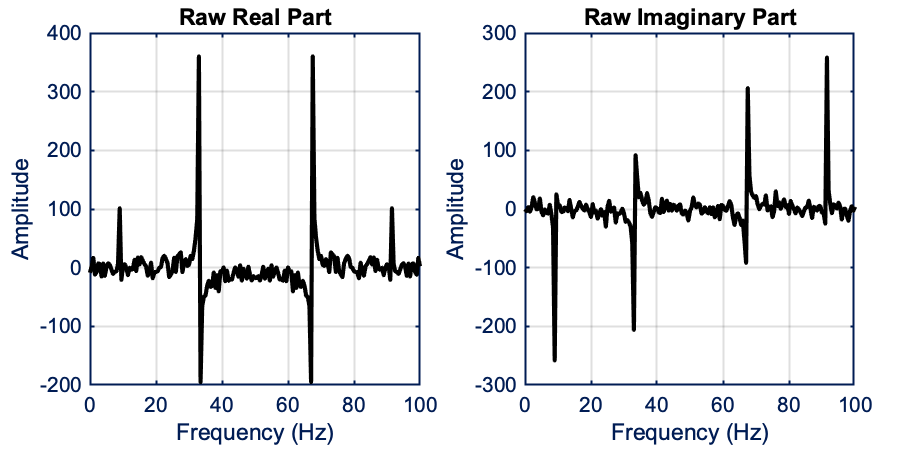
\includegraphics[width = 6 in]{Chapters/Signal Processing/Figures/Raw FFT Output.png}
    \caption{The raw output of the FFT function in MATLAB, showing both the real (left) and imaginary (right) parts of the output.}
    \label{fig:Raw FFT Output}
\end{figure}

Now we will turn our attention to only the real part.
We can now normalize the amplitudes by dividing the FFT output by the length of the waveform and taking the absolute value, as shown in Figure \ref{fig:Normalized Double-sided Spectrum}.
Notice that the amplitudes of the tones are incorrect.
To correct for this, we will take the right-hand side (everything greater than fs/2) and adding it on top of everything on the left-hand side.
More simply still, we can just get rid of the right-hand side and double the amplitudes of the left-hand side.
This result is shown in Figure \ref{fig:Normalized Single-sided Spectrum}.
Notice that we don't get the correct amplitudes. This can be fixed by using a higher sampling frequency, as shown in Figure \ref{fig:FFT Using a Higher Sampling Frequency}.

\begin{figure}[H]
    \centering
    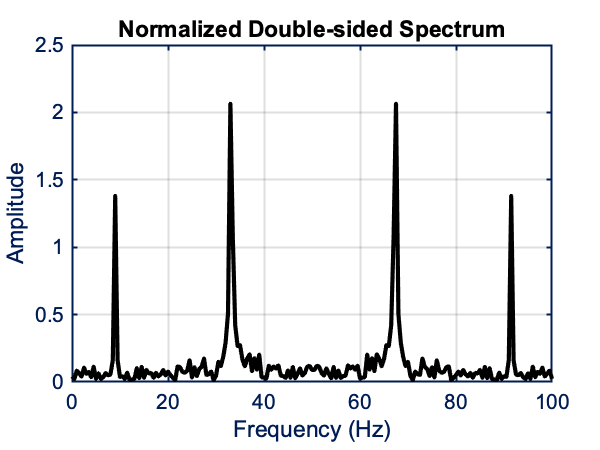
\includegraphics[width = 4 in]{Chapters/Signal Processing/Figures/Normalized Double-sided Spectrum.png}
    \caption{The normalized double-sided spectrum.}
    \label{fig:Normalized Double-sided Spectrum}
\end{figure}

\begin{figure}[H]
    \centering
    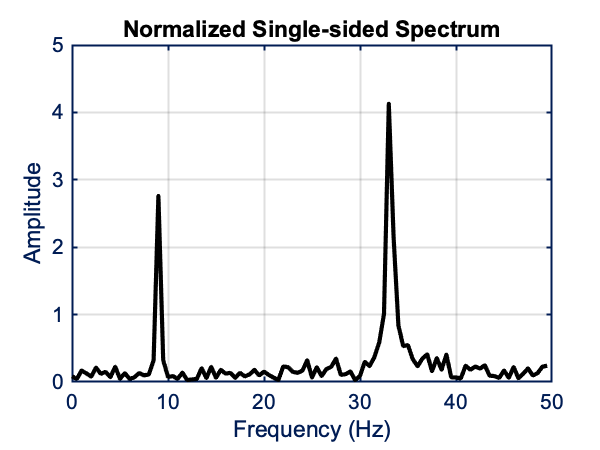
\includegraphics[width = 4 in]{Chapters/Signal Processing/Figures/Normalized Single-sided Spectrum.png}
    \caption{The normalized single-sided spectrum.}
    \label{fig:Normalized Single-sided Spectrum}
\end{figure}

\begin{figure}[H]
    \centering
    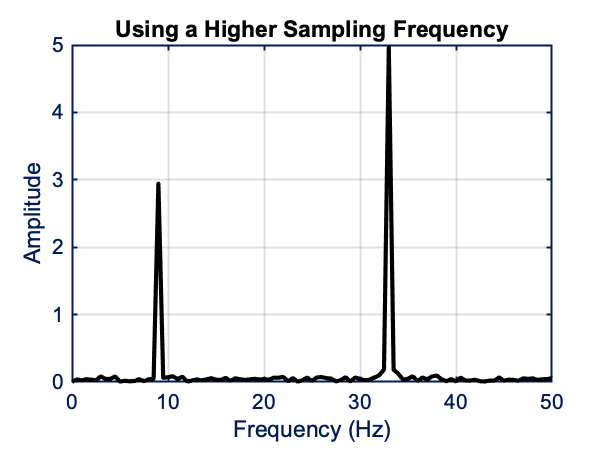
\includegraphics[width = 4 in]{Chapters/Signal Processing/Figures/Using a Higher Sampling Frequency.png}
    \caption{The normalized single-sided spectrum obtained using a sampling frequency of 1000 Hz instead of 100 Hz.}
    \label{fig:FFT Using a Higher Sampling Frequency}
\end{figure}

Lastly, the frequency resolution can be improved by increasing the length of the recording, as shown in Figure \ref{fig:Adjusting the Recording Length for FFT}.

\begin{figure}[H]
    \centering
    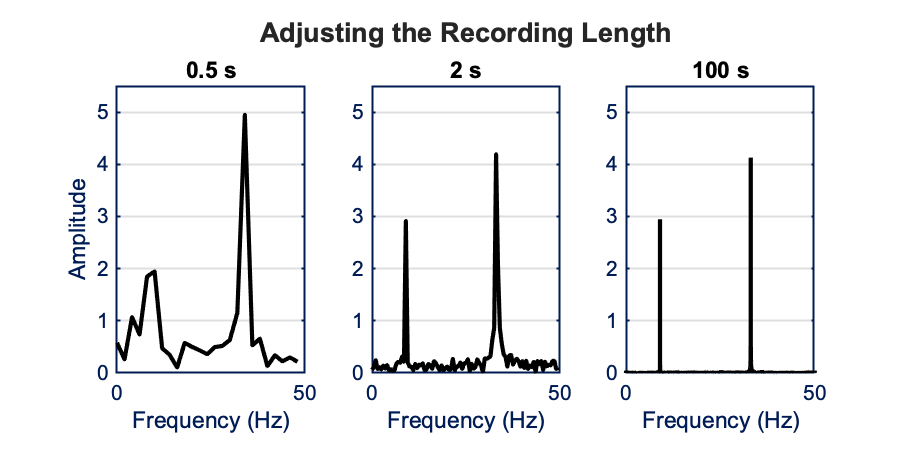
\includegraphics[width = 6 in]{Chapters/Signal Processing/Figures/Adjusting the Recording Length.png}
    \caption{The single-sided spectra calculated using a few different recording lengths. The frequency resolution increases with increased recording length.}
    \label{fig:Adjusting the Recording Length for FFT}
\end{figure}